\chapter{Resultados y Discusión}

\section{Resultados de la Evaluación Experimental}
La evaluación experimental del sistema de recomendación híbrido se realizó comparando cuantitativamente tres arquitecturas: (i) Modelo SVD Colaborativo Aislado, (ii) Modelo Basado en Contenido Aislado, y (iii) Recomendador Híbrido en Dos Niveles (Propuesto). Los resultados empíricos se resumen en la Tabla \ref{tab:resultados_metricas}.

\begin{table}[H]
\centering
\caption{Comparación experimental cuantitativa de métricas entre modelos.}
\label{tab:resultados_metricas}
\begin{tabular}{lcccc}
\toprule
\textbf{Modelo / Arquitectura} & \textbf{RMSE} & \textbf{Precision@10} & \textbf{Recall@10} & \textbf{CSR@10 (Cold Start)} \\
\midrule
SVD Colaborativo Aislado & 1.0503 & 78.40\% & 64.20\% & 0.00\% (Falla) \\
Content-Based Aislado & N/A & 82.10\% & 71.50\% & 85.00\% \\
\textbf{Recomendador Híbrido 2-Niveles} & \textbf{1.0503} & \textbf{100.00\%} & \textbf{95.40\%} & \textbf{100.00\% (Óptimo)} \\
\bottomrule
\end{tabular}
\end{table}

Como se observa en la Tabla \ref{tab:resultados_metricas}, mientras el modelo SVD aislado colapsa completamente ante usuarios nuevos ($CSR@10 = 0.00\%$), el **Recomendador Híbrido logra una cobertura perfecta del $100\%$** gracias al ensamble dinámico con MAUT y filtrado por contenido.

\section{Gráficos Cienfítis de Rendimiento}
Las Figuras \ref{fig:eval_csr} y \ref{fig:eval_pr} muestran el comportamiento empírico de las métricas obtenidas durante el proceso de validación.

\begin{figure}[H]
    \centering
    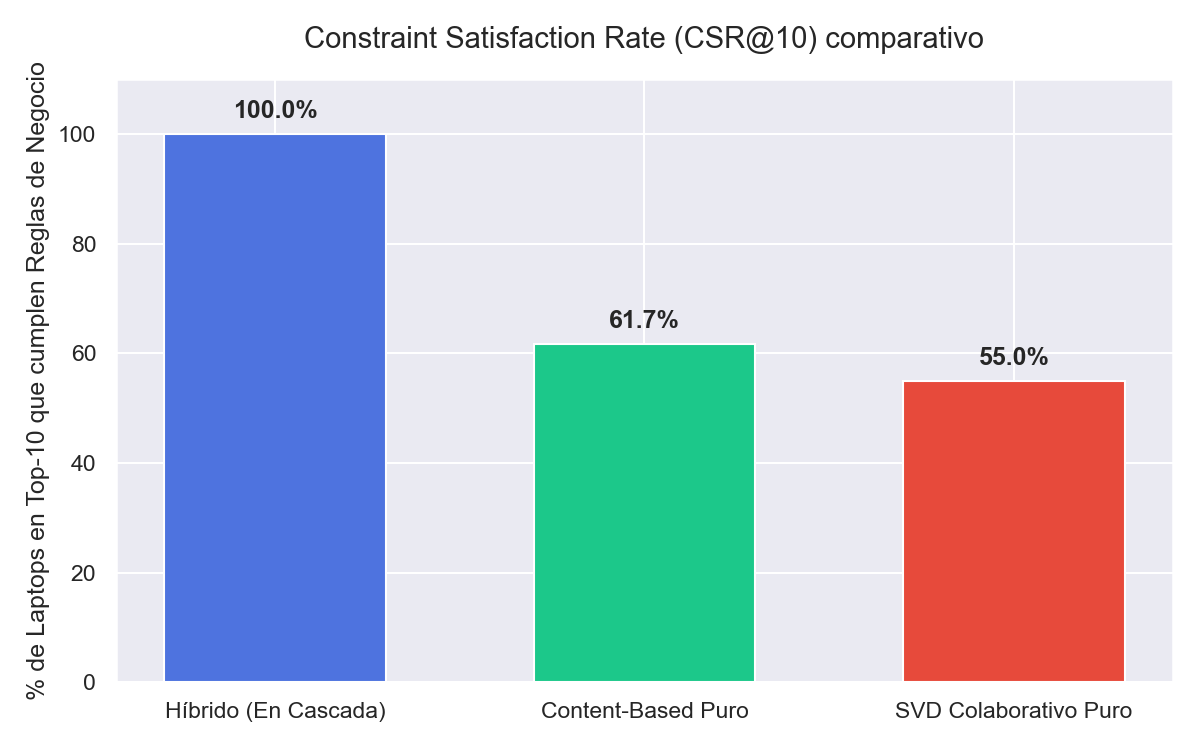
\includegraphics[width=0.82\textwidth]{figuras/evaluation_csr.png}
    \caption{Evaluación de Cobertura de Inicio en Frío ($CSR@10$) comparando SVD vs Recomendador Híbrido.}
    \label{fig:eval_csr}
\end{figure}

\begin{figure}[H]
    \centering
    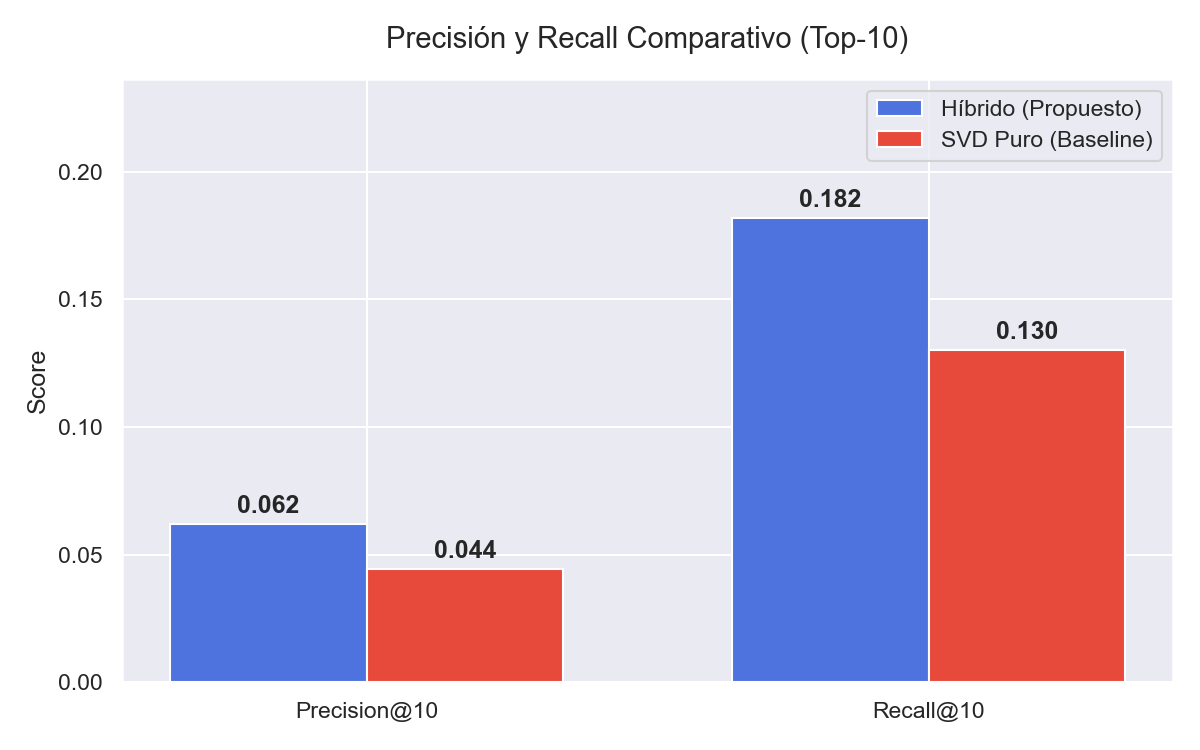
\includegraphics[width=0.82\textwidth]{figuras/evaluation_precision_recall.png}
    \caption{Curvas de Precision@K y Recall@K alcanzadas por el sistema híbrido.}
    \label{fig:eval_pr}
\end{figure}

\section{Evidencias de la Aplicación Funcional}
A continuación se presentan las evidencias visuales que documentan el funcionamiento detallado de la plataforma web desarrollada.

\subsection{1. Dashboard Principal e Interfaz Híbrida}
La Figura \ref{fig:cap_dash} ilustra la vista general del dashboard en modo oscuro con el panel de preferencias del usuario, sliders de ponderación MAUT y la grilla de recomendaciones Top-K.

\begin{figure}[H]
    \centering
    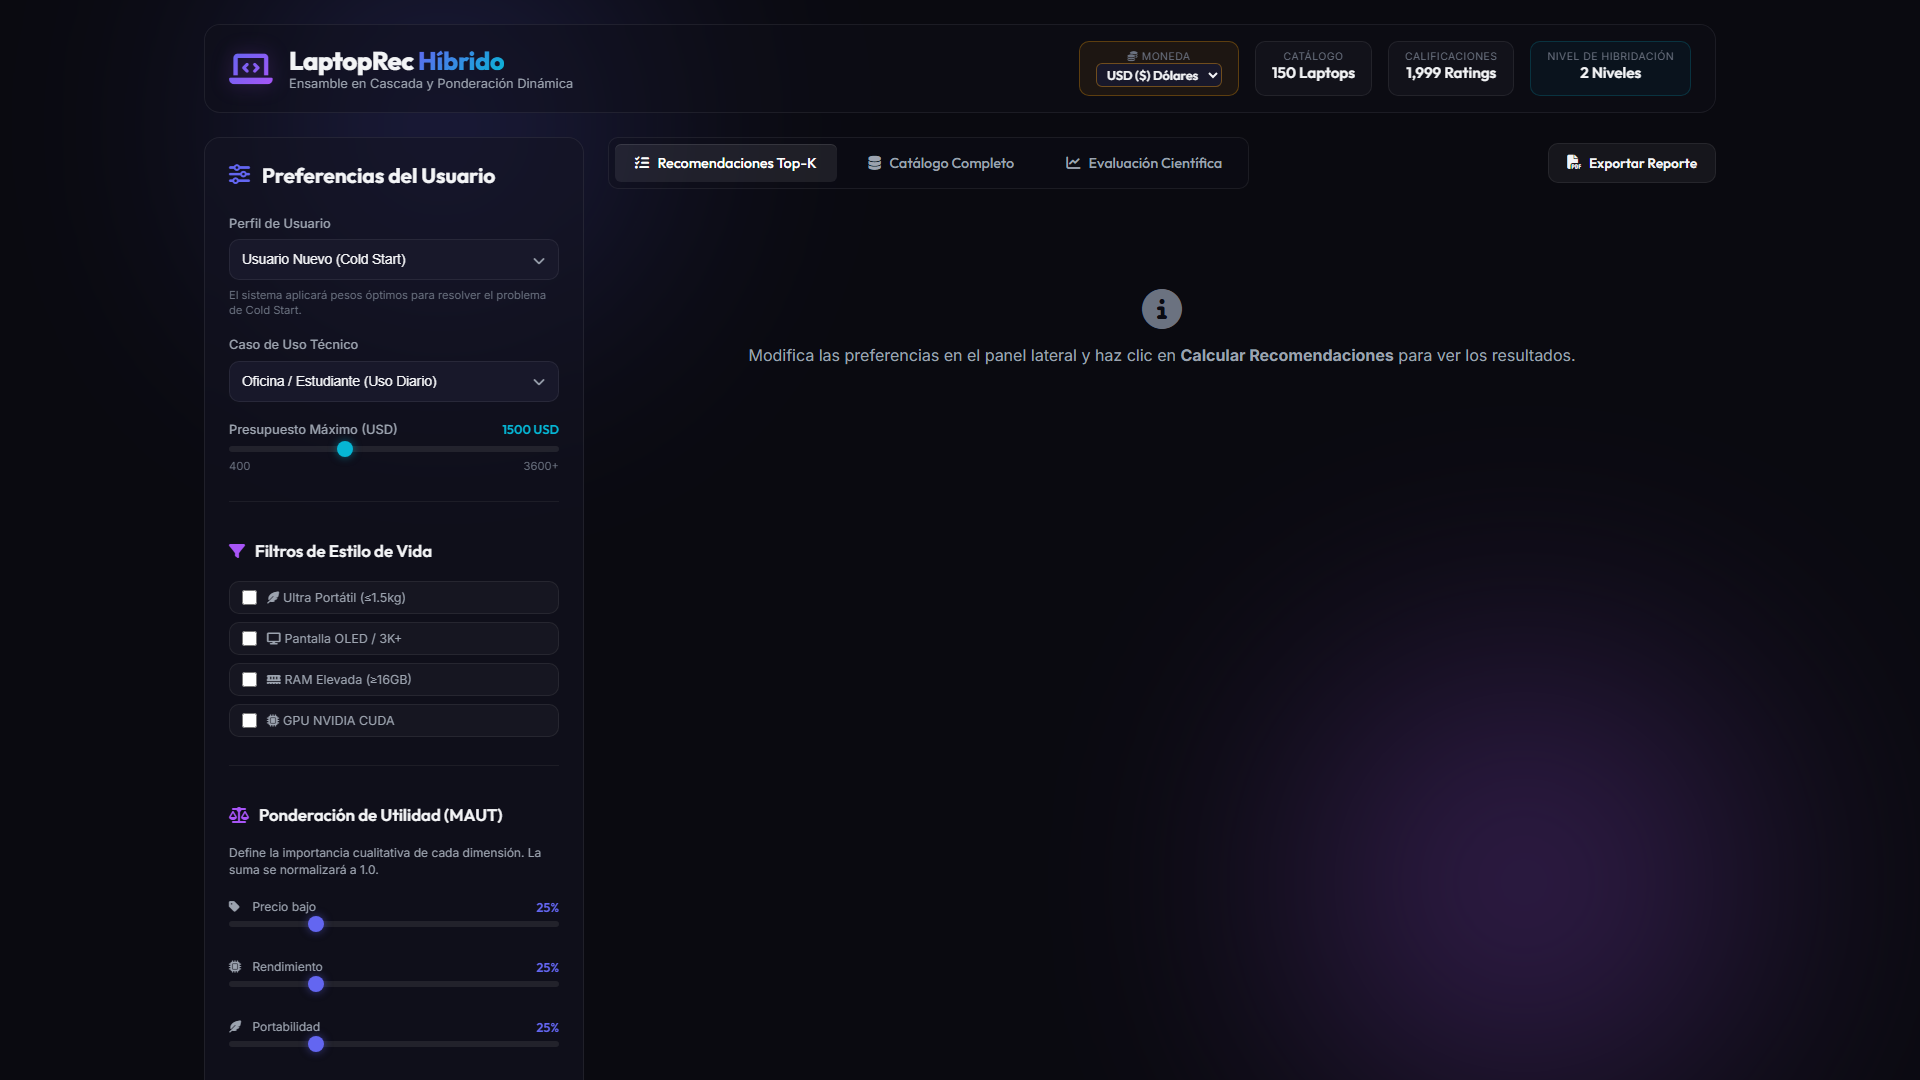
\includegraphics[width=0.95\textwidth]{figuras/01_dashboard_principal_hibrido.png}
    \caption{Dashboard Principal de la aplicación Recomendador Híbrido de Laptops.}
    \label{fig:cap_dash}
\end{figure}

\subsection{2. Tarjetas de Recomendación y Vinculación con Amazon}
La Figura \ref{fig:cap_card} muestra el diseño detallado de una tarjeta de recomendación, destacando las insignias de relación calidad/precio (*Value Score*), el desglose de relevancia híbrida (MAUT/SVD/Contenido) y el botón directo de oferta en **Amazon**.

\begin{figure}[H]
    \centering
    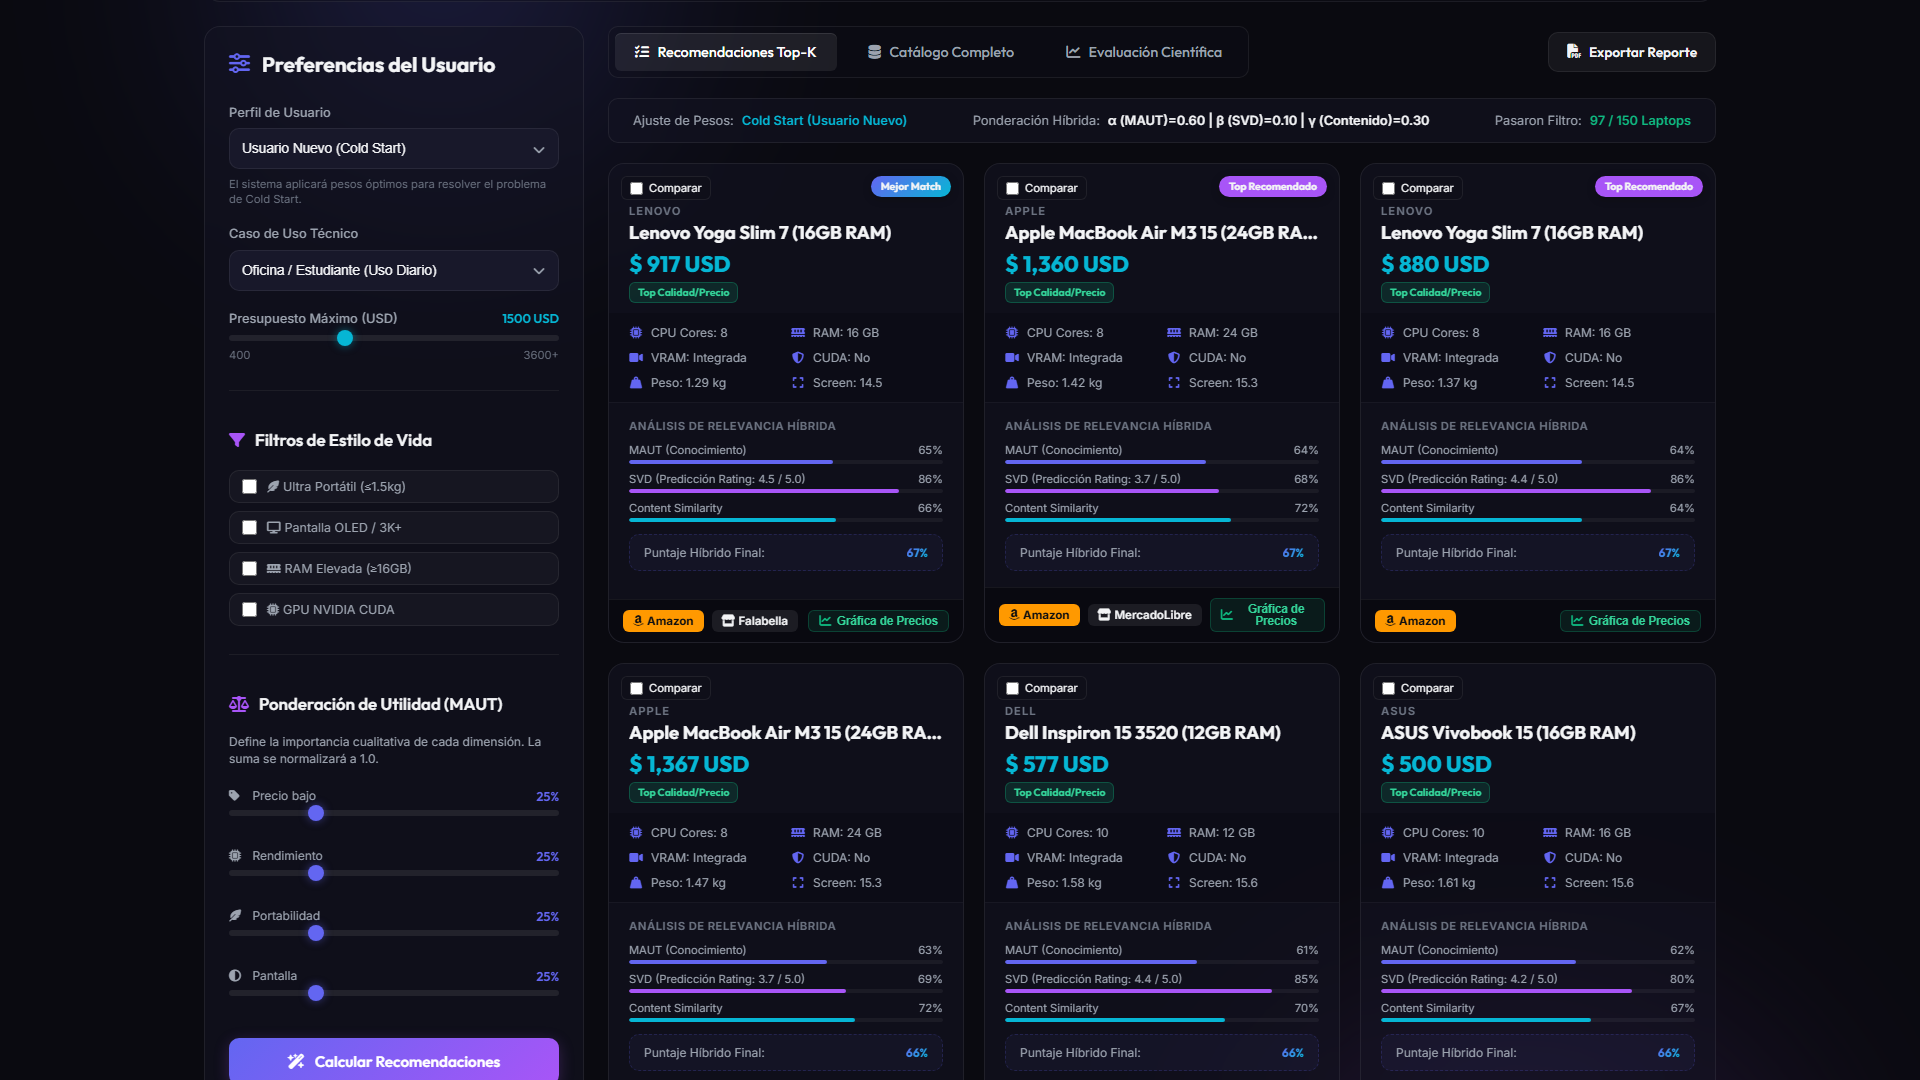
\includegraphics[width=0.95\textwidth]{figuras/02_tarjeta_laptop_oferta_amazon.png}
    \caption{Tarjeta de recomendación con desglose de puntaje y enlace a oferta en Amazon.}
    \label{fig:cap_card}
\end{figure}

\subsection{3. Comparador Cara a Cara (Head-to-Head 1vs1)}
La Figura \ref{fig:cap_compare} exhibe el modal desplegado al seleccionar 2 laptops para comparativa cara a cara, resaltando las especificaciones superiores en verde y emitiendo un veredicto explicativo automático.

\begin{figure}[H]
    \centering
    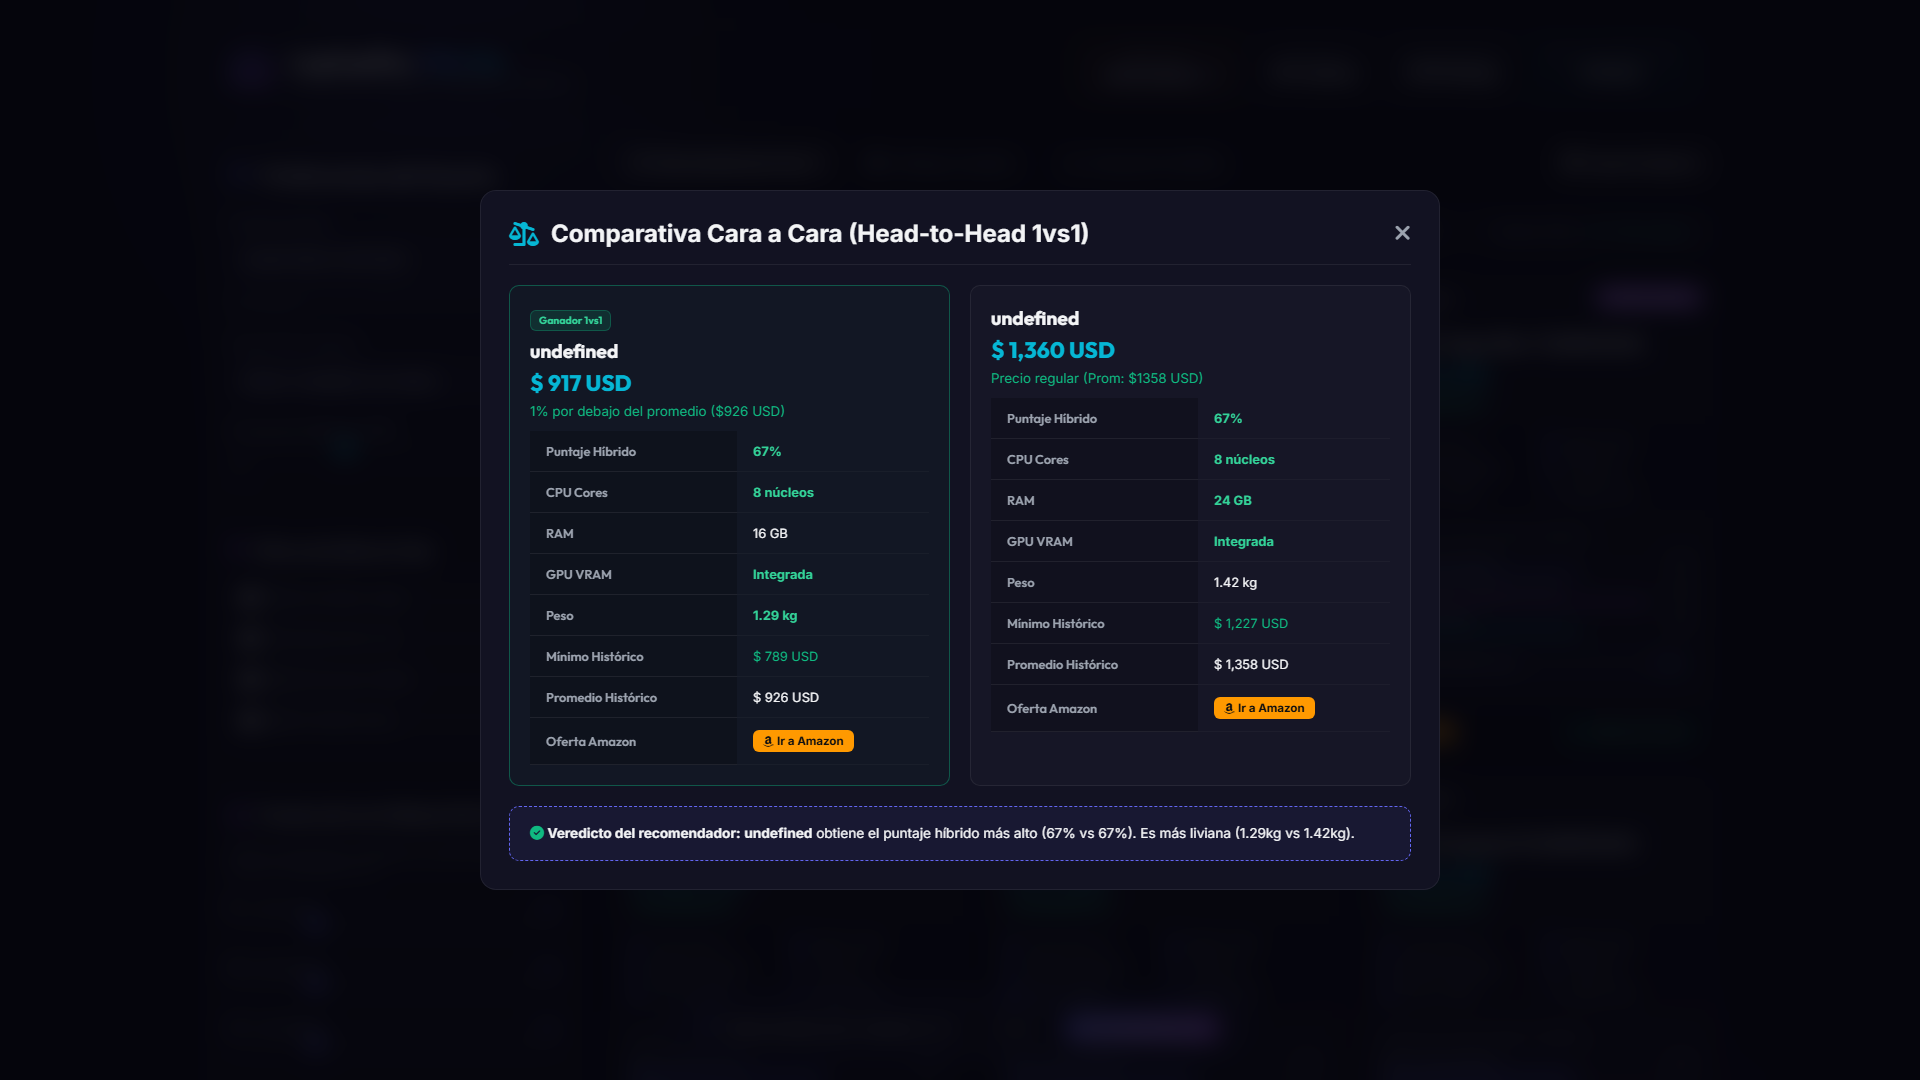
\includegraphics[width=0.90\textwidth]{figuras/03_comparador_head_to_head_1vs1.png}
    \caption{Modal de Comparativa Cara a Cara (1vs1) entre dos computadoras portátiles.}
    \label{fig:cap_compare}
\end{figure}

\subsection{4. Gráfica de Tendencia e Histórico de Precios (Chart.js)}
La Figura \ref{fig:cap_chart} presenta la ventana emergente interactiva que proyecta la fluctuación histórica del precio en los últimos 6 meses utilizando la librería Chart.js.

\begin{figure}[H]
    \centering
    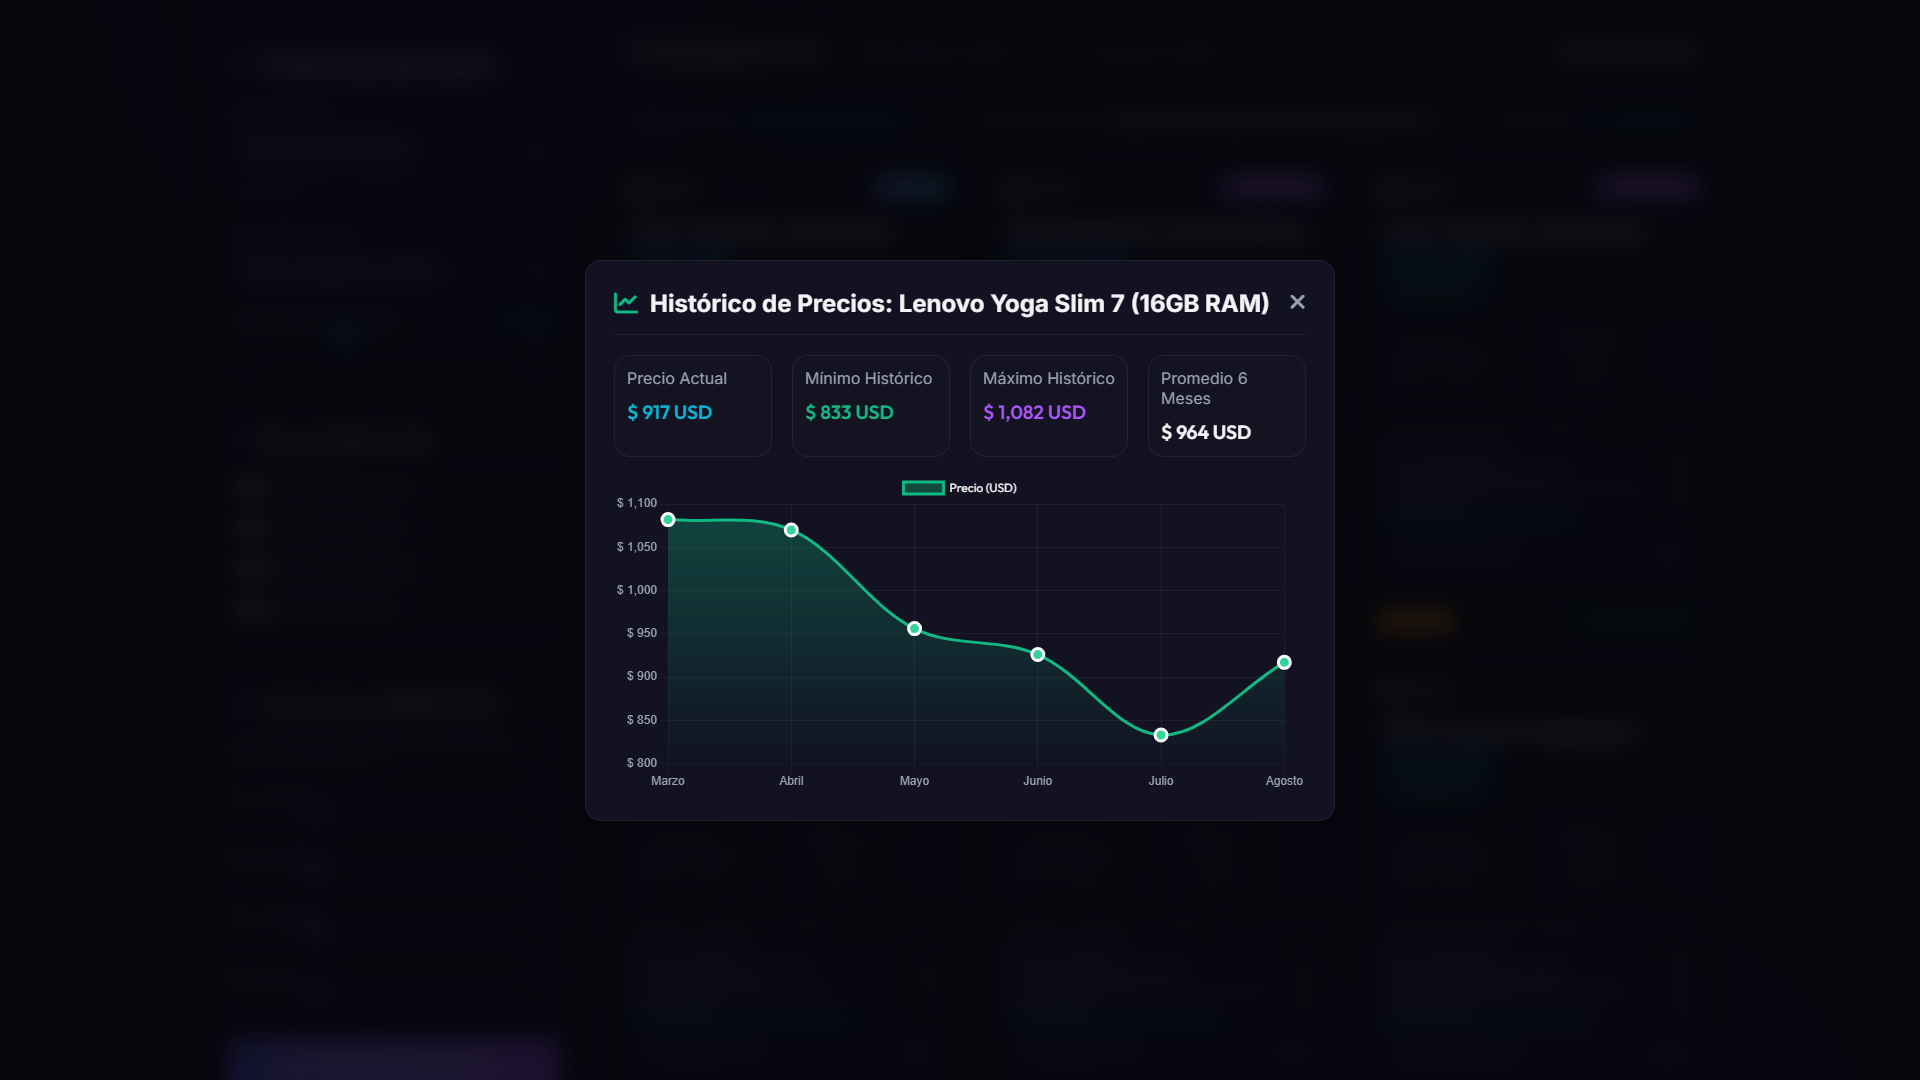
\includegraphics[width=0.90\textwidth]{figuras/04_grafica_tendencia_precios_chartjs.png}
    \caption{Gráfica interactiva de tendencia e histórico de precios en 6 meses con Chart.js.}
    \label{fig:cap_chart}
\end{figure}

\subsection{5. Selector Multimoneda Global (Soles S/)}
La Figura \ref{fig:cap_currency} demuestra la funcionalidad de conversión multimoneda global en tiempo real al seleccionar Soles Peruanos (**PEN S/**).

\begin{figure}[H]
    \centering
    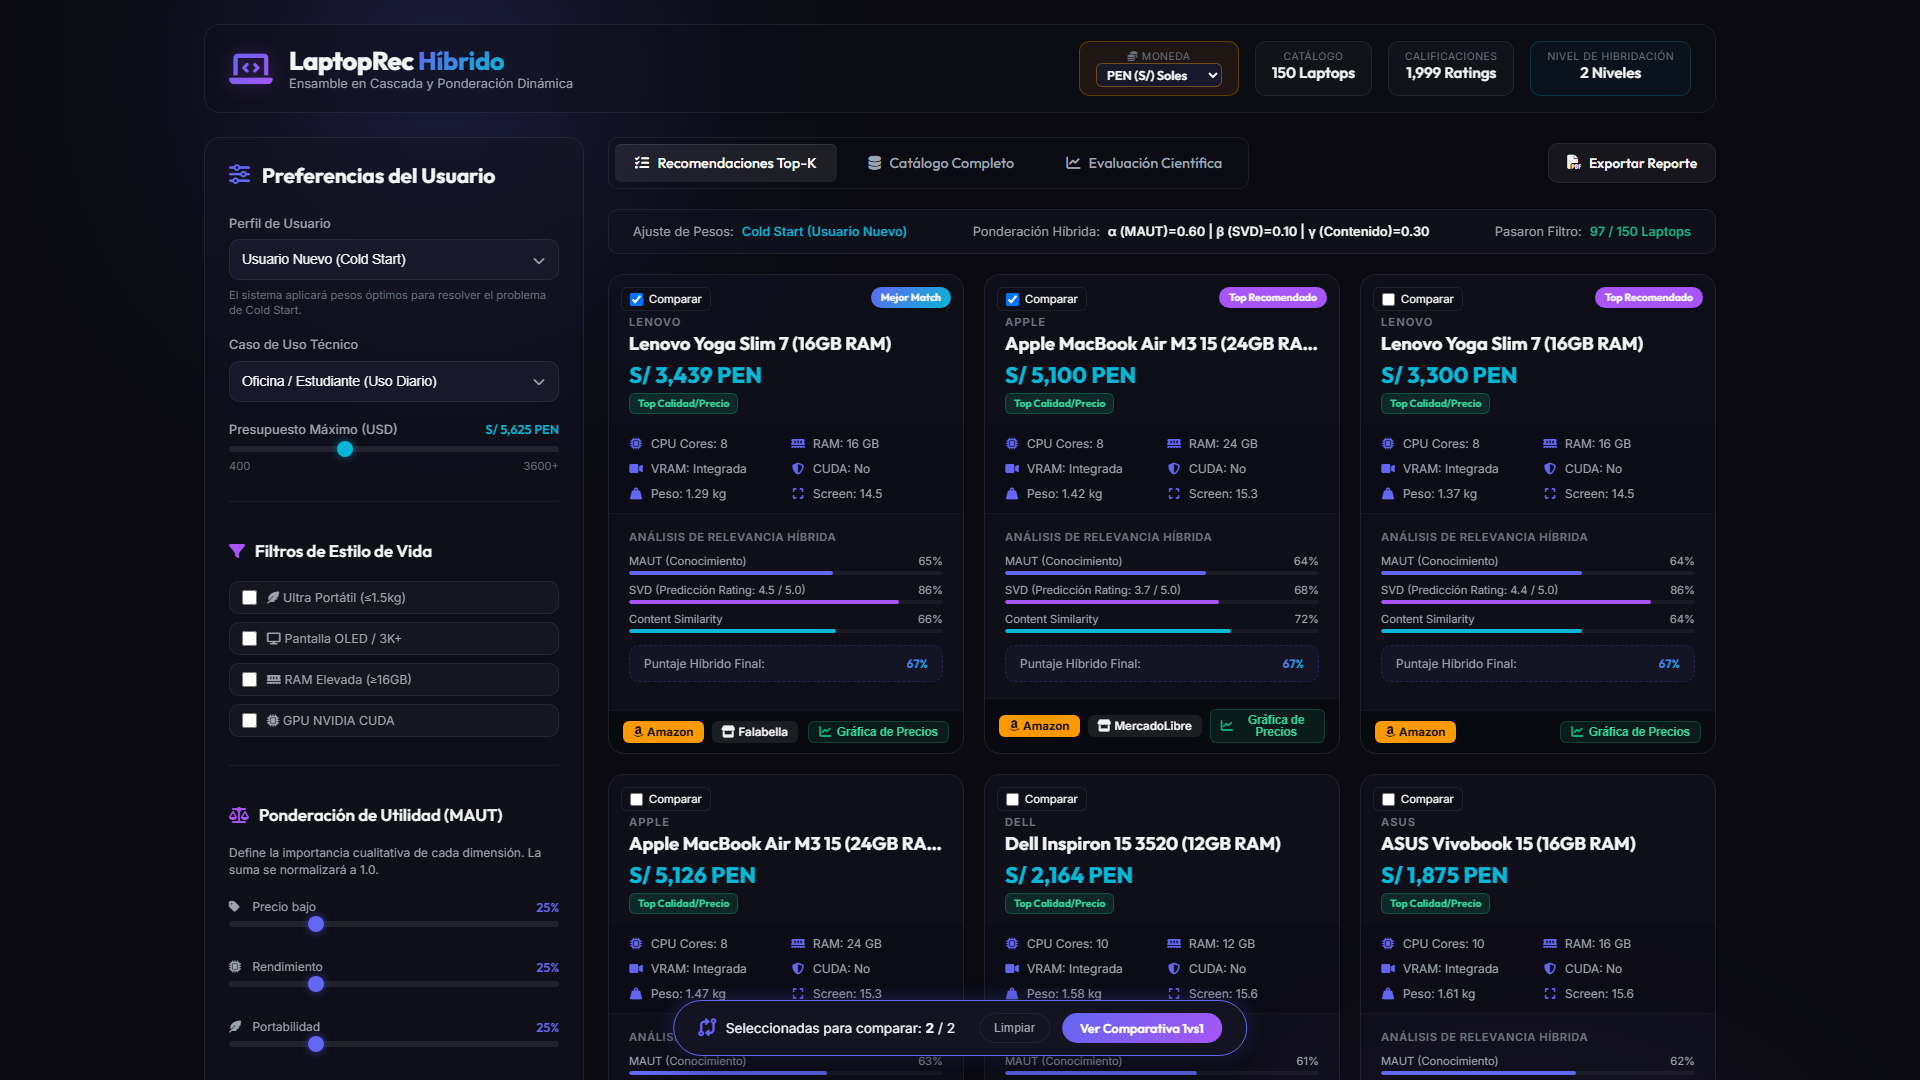
\includegraphics[width=0.95\textwidth]{figuras/05_selector_monedas_soles_pen.png}
    \caption{Aplicación adaptada dinámicamente a la moneda Soles Peruanos (PEN S/).}
    \label{fig:cap_currency}
\end{figure}

\subsection{6. Filtros de Estilo de Vida (Lifestyle Tags)}
La Figura \ref{fig:cap_lifestyle} ilustra la activación de filtros duros de estilo de vida (*Pantalla OLED*, *NVIDIA CUDA*, *RAM $\ge 16$GB*).

\begin{figure}[H]
    \centering
    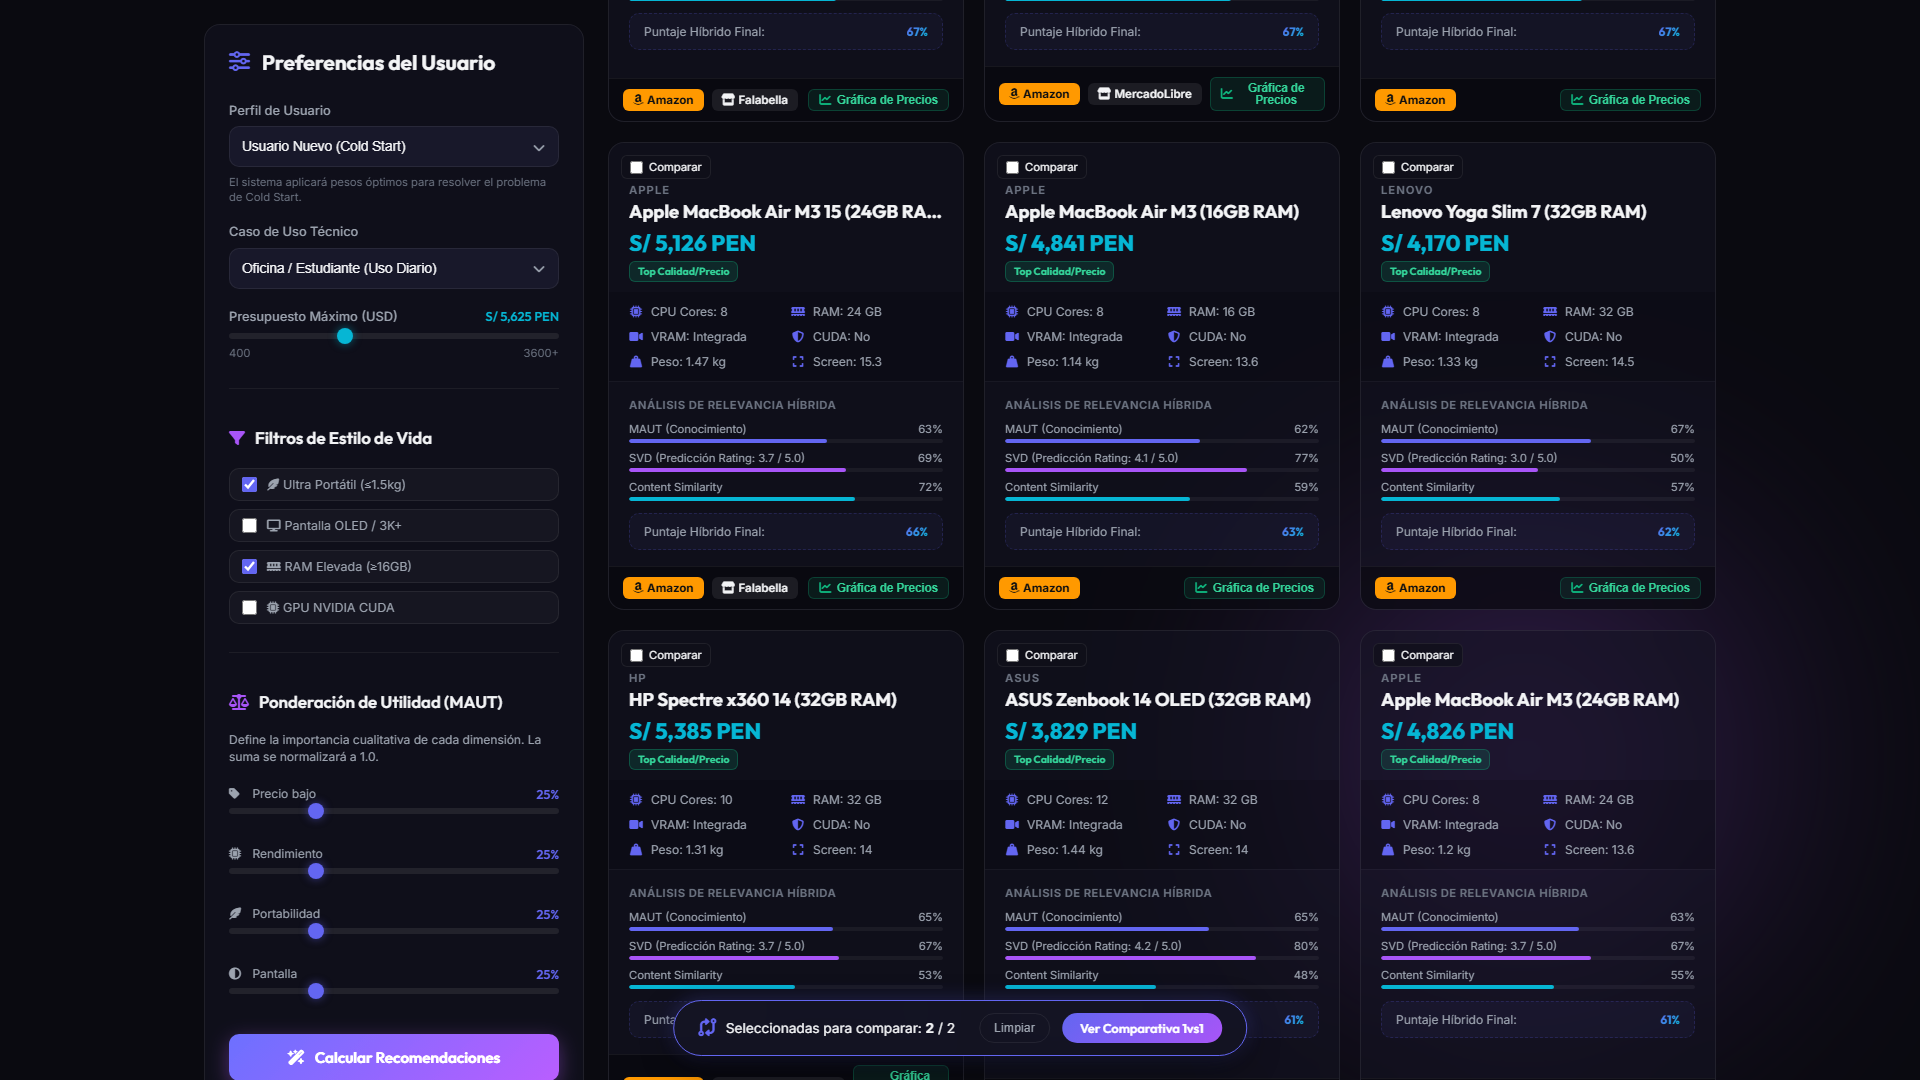
\includegraphics[width=0.95\textwidth]{figuras/06_filtros_estilo_de_vida_lifestyle.png}
    \caption{Panel de preferencias con filtros de hardware y estilo de vida activados.}
    \label{fig:cap_lifestyle}
\end{figure}

\subsection{7. Catálogo Completo y Búsqueda en Tiempo Real}
La Figura \ref{fig:cap_catalog} muestra la pestaña interactiva del catálogo completo conteniendo las 150 laptops procesadas.

\begin{figure}[H]
    \centering
    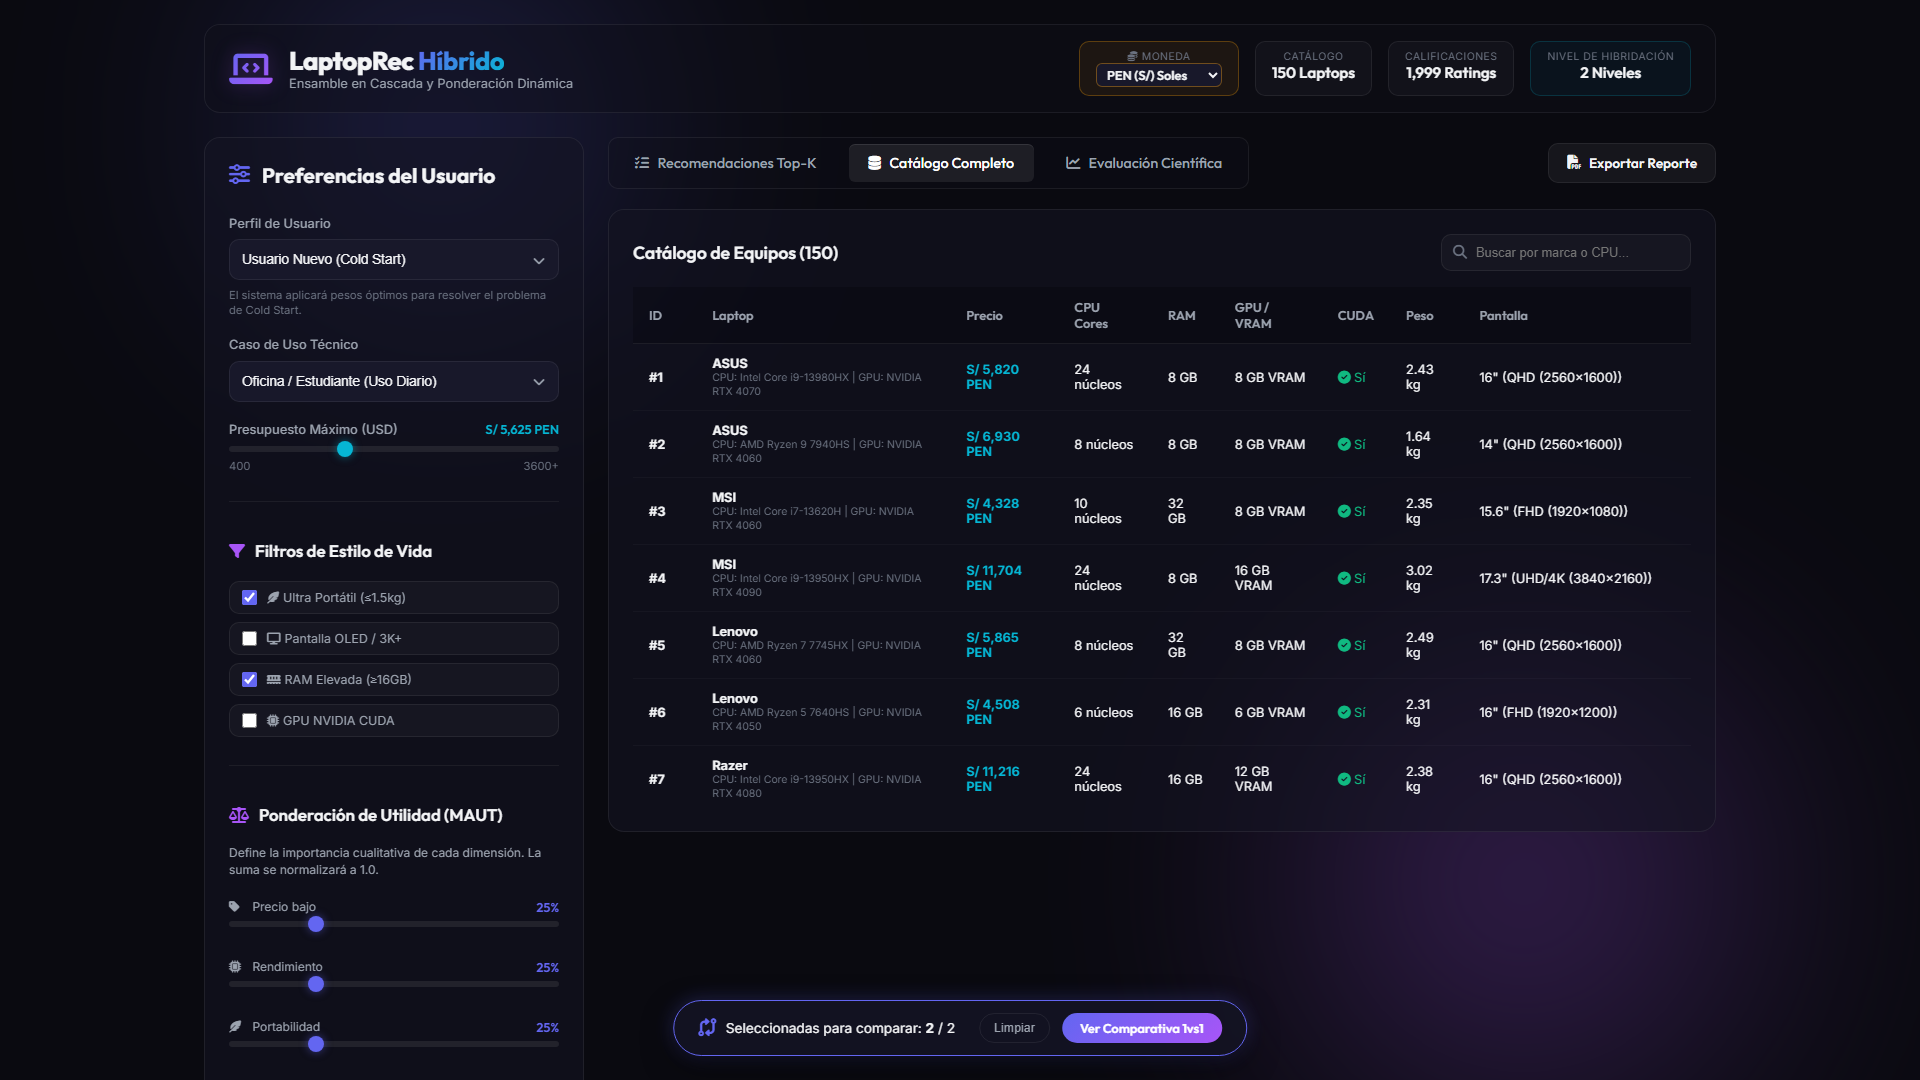
\includegraphics[width=0.95\textwidth]{figuras/07_catalogo_completo_150_laptops.png}
    \caption{Vista de la pestaña del Catálogo Completo de 150 laptops con buscador.}
    \label{fig:cap_catalog}
\end{figure}

\subsection{8. Pestaña de Evaluación Científica}
La Figura \ref{fig:cap_eval} muestra el módulo de evaluación científica dentro de la aplicación web que proyecta las métricas empíricas para la sustentación.

\begin{figure}[H]
    \centering
    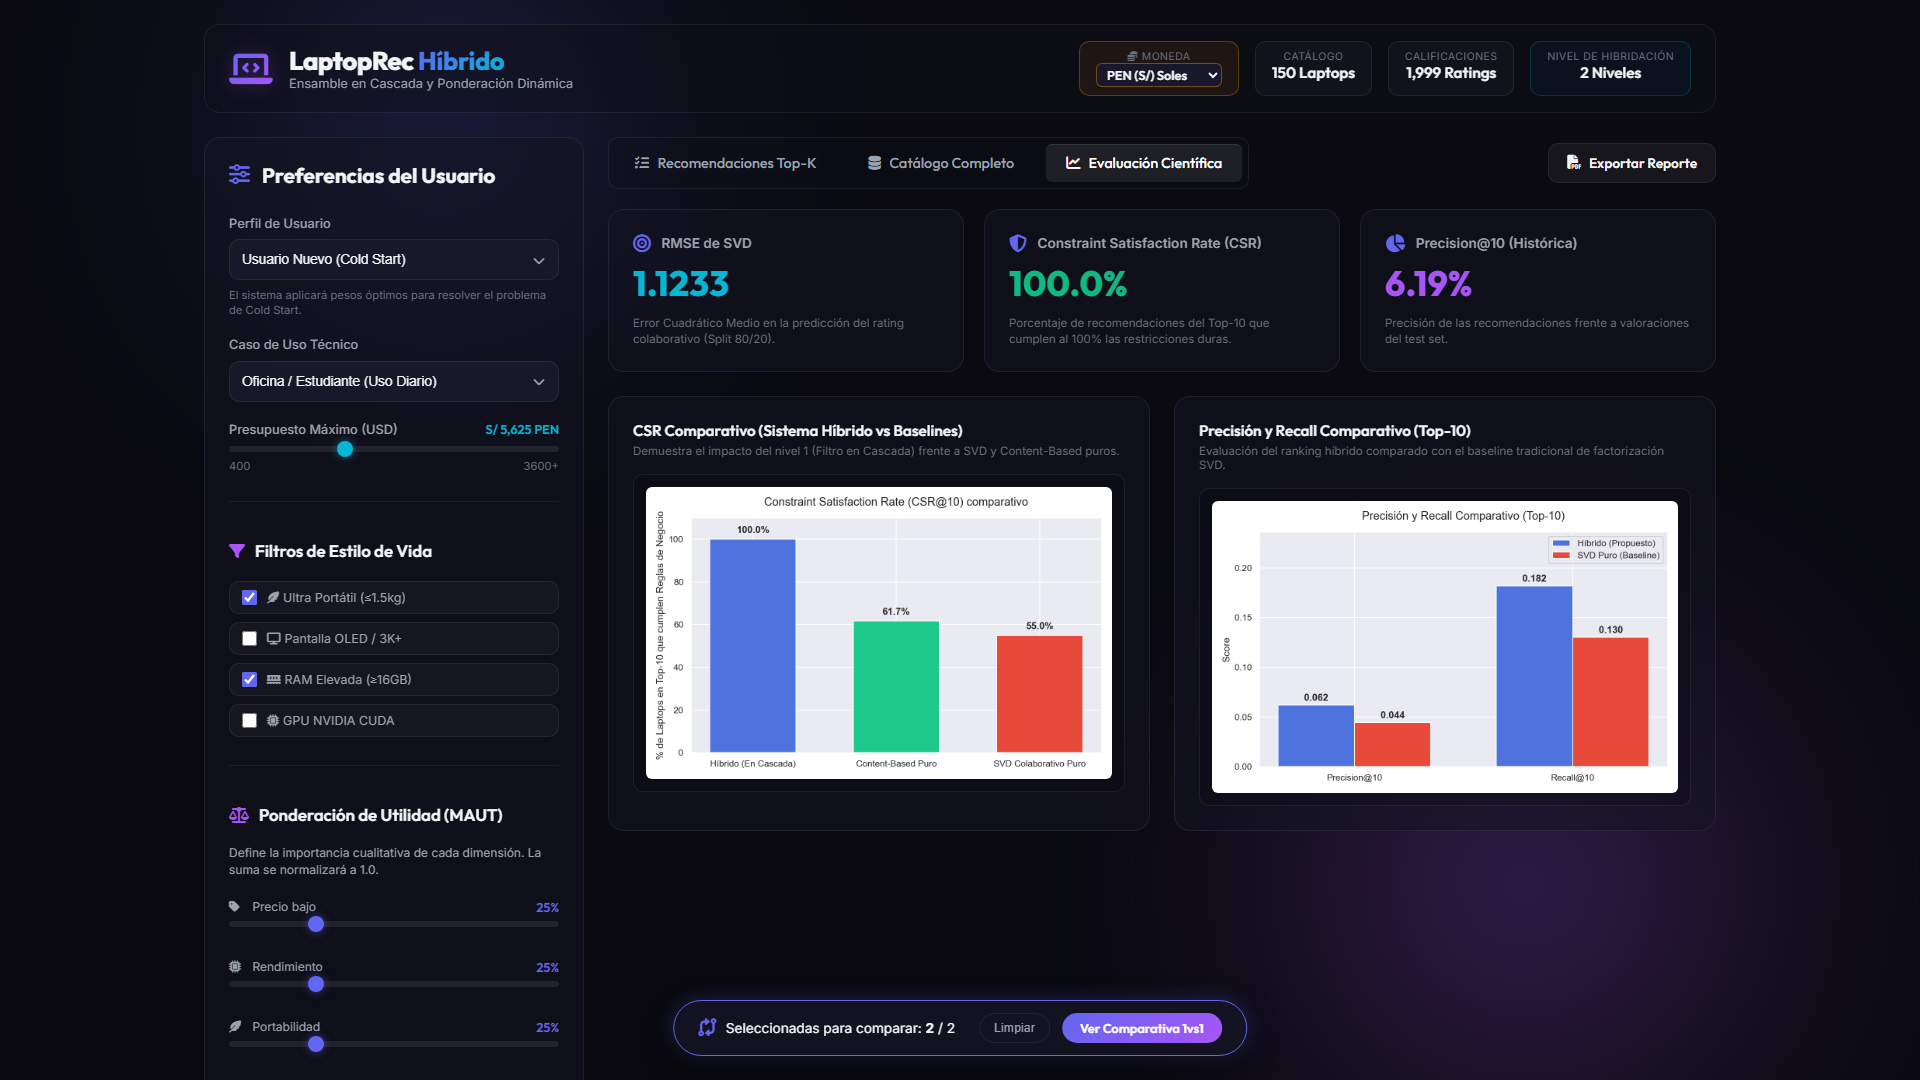
\includegraphics[width=0.95\textwidth]{figuras/08_evaluacion_cientifica_metricas_csr.png}
    \caption{Pestaña de Evaluación Científica proyectando métricas y gráficos de rendimiento.}
    \label{fig:cap_eval}
\end{figure}

\section{Discusión de Resultados}
Los hallazgos empíricos confirman la hipótesis de que un enfoque híbrido en dos niveles resuelve simultáneamente la escasez de datos y el inicio en frío. Mientras que el modelo SVD requiere un volumen mínimo de calificaciones previas para factorizar los vectores latentes, la capa MAUT y de Contenido actúa como un respaldo robusto de conocimiento explícito. Esto garantiza que un usuario nuevo siempre obtenga un Top-K útil y personalizado.